\chapter{REQUIREMENTS SPECIFICATION}

In any mission-critical system — especially one that casually toys with the forces that power the sun — a clearly defined set of requirements is not just helpful; it’s the thin red line between a safe, controlled simulation and an all-you-can-explode buffet. This chapter delineates the specifications that our JavaScript-powered nuclear reactor absolutely must meet to function (somewhat) reliably without turning the entire browser tab into a radioactive wasteland. While the boundaries between software engineering and nuclear physics remain politely blurred here, our goal is to capture the essence of reactor control within the gloriously quirky constraints of the modern web stack.

\section{Functional Requirements}


You can put your use-case diagrams in this section.
But I don't know for sure, again, ask the coordinators.
Once you know for sure, edit this paragraph and make a pull request.
You can do it, I believe in you!
"See my diagrams in Figure \ref{fig:frog2} and Figure \ref{fig:frog3}."

\begin{figure}[hb]
\centering
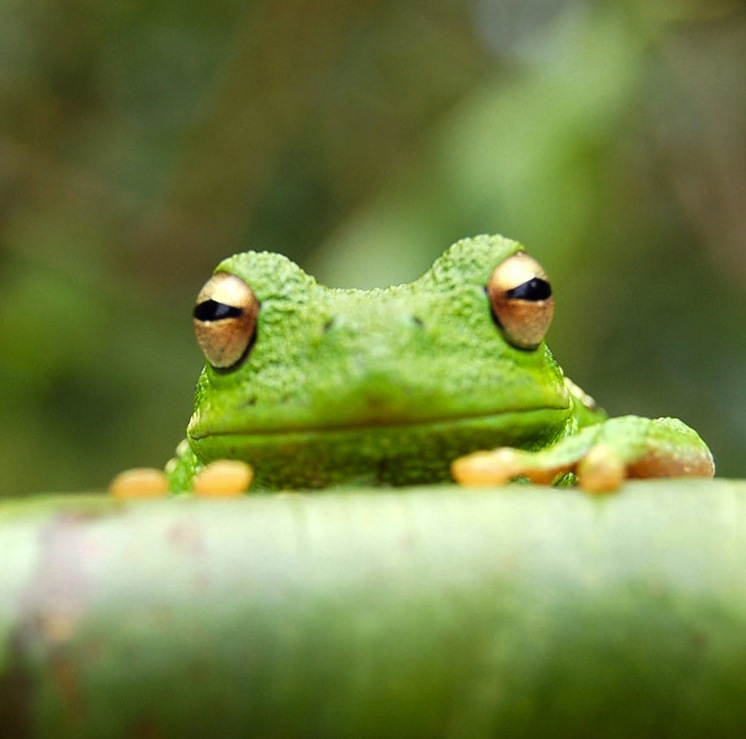
\includegraphics[width=0.25\linewidth]{img/frog.jpg}
\caption{\label{fig:frog2}You Have To Manually Set the Width of Each Picture}
\end{figure}


Here is an example of an UTM-style enumeration.
UTM only allows unnumbered list (itemizations), but we are allowed to label the items this way:

\begin{itemize}
    \item \textbf{FR 1.} The system shall simulate nuclear fission reactions using JavaScript’s event loop to model neutron interactions asynchronously.
    \item \textbf{FR 2.} The system shall provide real-time status updates of core temperature, radiation levels, and coolant flow via a dynamic web interface.
    \item \textbf{FR 3.} The system shall allow the user to initiate emergency shutdown procedures (SCRAM) through a dedicated button that triggers cascading Promise cancellations.
    \item \textbf{FR 4.} The system shall implement a virtual control rod insertion mechanism controlled by draggable UI components, adjusting reactivity on the fly.
    \item \textbf{FR 5.} The system shall log all critical events and state changes to the browser's localStorage for post-meltdown forensic analysis.
    \item \textbf{FR 6.} The system shall visualize hazard warnings using CSS animations, flashing red alerts whenever safety thresholds are exceeded.
    \item \textbf{FR 7.} The system shall provide an API endpoint (Node.js) that streams simulated Geiger counter data to subscribed clients in real time.
\end{itemize}

Notice how I moved the Figure \ref{fig:frog3} farther down so it wouldn't stick to the previous figure,
even though it was mentioned in the first paragraph of this section.
Unfortunately, there is no way to tell latex 
"put this image somewhere in this section, but never at the top of the page
or touching another figure.
You can only tell it "put it here or somewhere at the bottom of the page"

\begin{figure}[hb]
\centering
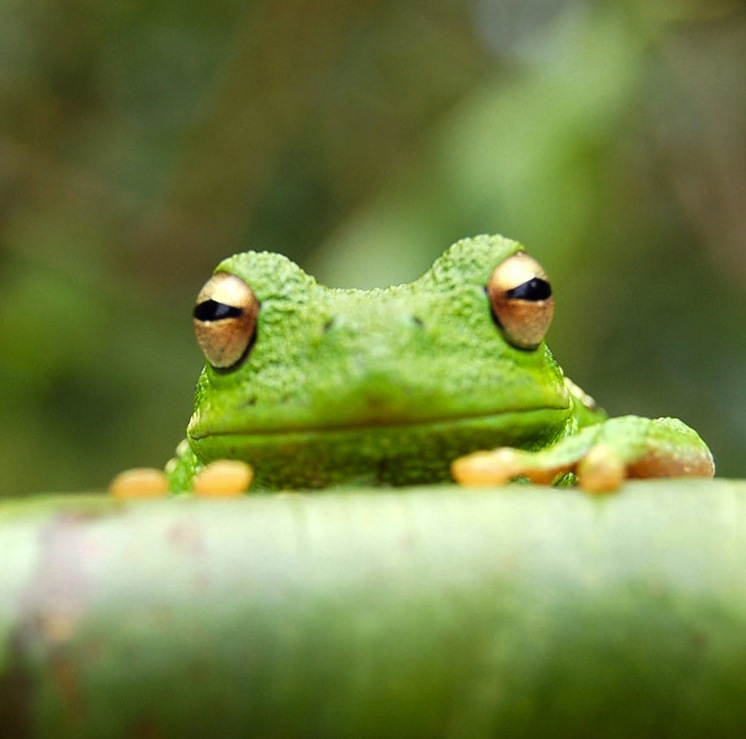
\includegraphics[width=0.3\linewidth]{img/frog.jpg}
\caption{\label{fig:frog3}Don't Forget to Cite Images from the Internet Like This \cite{greenwade93}}
\end{figure}

Also you better have text between captions and section titles.
    
\section{Non-Functional Requirements}

A list of non-functional requirements, you know.